\chapter{Hardware}
\label{sec:Hardware}
\todo{Besseres Bild! Schema? Bessere Beschriftung!}
\begin{figure}[htb]
\centering
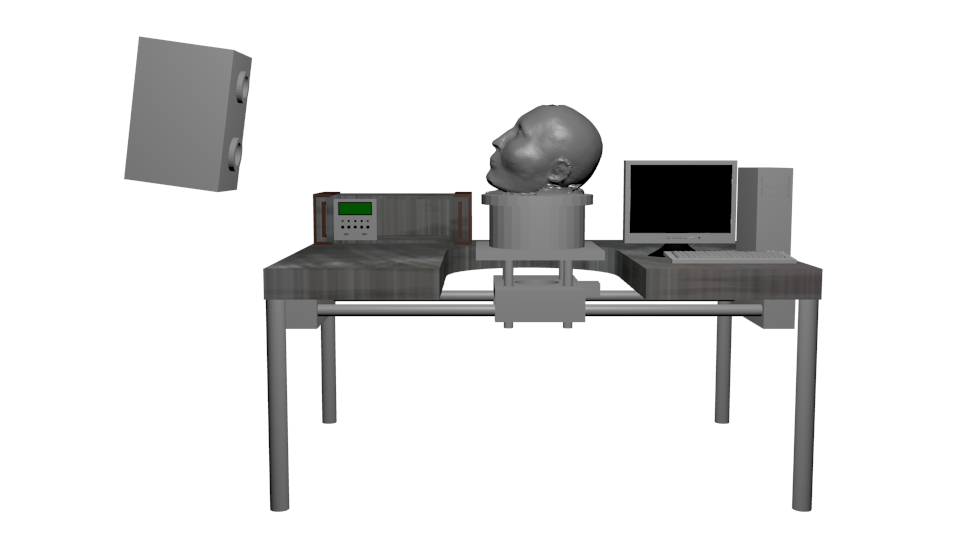
\includegraphics[width=\textwidth]{Blender/Schema_Arbeitsplatz.png}
\caption{Überblick des Arbeitsplatz}
\label{fig:Übersicht}
\end{figure}

\todo{ Fußnoten für Komponenten, Herst. u. Websites}\\
\todo{ Komponenten auf Abbildung erwähnen!}

\section{Lasererfassungssystem VI-900}
\todo{Bild}
Das Lasererfassungssystem \Fachbegriff{VI-900} der Firma \Fachbegriff{Minolta} besteht aus einem \Fachbegriff{Lasertriangulator} und einer Kamera. Das System lässt sich über eine \Fachbegriff{SCSI}-Schnittstelle ansprechen und konfigurieren. Zur mobilen Nutzung kann das Gerät auch auf der Rückseite bedient werden. Aufgenommene Daten können auf einer \Fachbegriff{CF-Karte} gespeichert werden. Im Projekt wurde jedoch lediglich die Ansteuerung via SCSI genutzt.

\section{Ansteuerung für den Drehtisch}
\subsection{Drehtisch}
Der Drehtisch ist eine Eigenkonstruktion der Werkstatt des RheinAhrCampus. Er besteht aus einer massiven Edelstahl Arbeitsplatte, welche auf 4 Füßen ruht. Aus dieser ist ein Rechteck mit aufgesetztem Halbkreis ausgeschnitten. In diesem Ausschnitt befindet sich der Drehtisch. Er ist auf einem Schienensystem gelagert. Mit dem Schienensystem lässt der Drehtisch sich in der Vertikalen positionieren. Mit einem Schrittmotor lässt sich der Drehtisch sich zusätzlich in der Höhe verstellen. Die Höhenverstellung wird mit einem Schneckengetriebe realisiert. Ein weiterer Schrittmotor ist für die Drehung des Tisches zuständig. Der Tisch ist über ein \Fachbegriff{Harmonic-Drive-Getriebe} mit dem Schrittmotor verbunden. Das Übersetzungsverhältnis beträgt 1:50.   
\subsection{Spannungsversorgung}
\todo{Verkabelung Steckbar und universell gemacht}
Die Schrittmotorkarten werden von einem PC-Netzteil gespießt. Die Kabel waren direkt an die Verbindungsleisten gelötet. Um den Aufbau modular und erweiterbar zu machen, ersetzte ich die feste Lötverbindung durch eine Standard PC-Netzteil Verbindung. Dadurch kann das Netzteil einfach ausgebaut werden, bzw. das System leicht mit neuen Einschubkarten erweitert werden.
\subsection{Schrittmotoren}
\todo{Motoren beschreiben! Technische Daten! Schritte, Spannungen. Verdrahtung.}
\subsection{Schrittmotorkarten}
Die Ansteuerung für die Schrittmotoren sind als 19"-Einschübe realisiert. Für jeden Schrittmotor wird ein Einschub benötigt.
Die Einschübe sind Produkte der Firma R+S. Mittels RS-232 Schnittstelle lassen sich die Karten konfigurieren und ansteuern. Die Konfiguration und Ansteuerung erfolgt über einen vorgegeben 
\Fachbegriff{ASCII} Befehlssatz. Der Befehlssatz befindet sich im Kapitel \ref{sec:A_ASCII_Befehle}.Es können 2 oder mehr Karten als 
\Fachbegriff{Daisy-Chain} 
\footnote{Als Daisy Chain (englisch, wörtlich „Gänseblümchenkette“) bezeichnet man eine Anzahl von Hardware-Komponenten, welche in Serie miteinander verbunden sind (meist in sogenannten Bussystemen in der Automatisierungstechnik).\cite{wiki:Daisy} } 
in Reihe geschaltet werden.
\subsection{Motorverkabelung}
Die Schrittmotoren benötigen ein mindestens 4-adriges Kabel. Das Kabel für den Schrittmotor der für die Rotation zuständig ist war bereits gefertigt. Das Kabel für den Schrittmotor der für die Höhenverstellung zuständig ist habe ich selbst gefertigt. Hier wurden 3 weitere Adern für die beiden Endschalter benötigt.
\todo{Schemazeichnung Kabel!}
\subsection{Endschalter}
Die Schrittmotorkarten unterstützen das Abschalten der Motoren wenn ein sogenannter Endschalter ausgelöst wird. Dies sind im allgemeinen mechanische Schalter die ausgelöst werden wenn der Tisch sich dem Ende des Arbeitsbereiches nähert. Dies verhindert eine Beschädigung des Aufbaus.\\
Im Aufbau waren bereits induktive Endschalter der Firma Pepperl+Fuchs verbaut. 
Normalerweise unterstützt die Schrittmotorkarte nur mechanische Endschalter. Durch geschickte Verdrahtung ließen sich die induktiven Endschalter verwenden. Hierzu musste über einen Spannungsteiler die Spannung herabgesetzt werden und konnte somit direkt an den Optokoppler der Schrittmotorkarte angeschlossen werden. \todo{Schemazeichnung der Verdrahtung}\\
Am Drehtisch war ein Metallstutzen angebracht der den Endschalter auslösen sollte. Dieser war jedoch ungeeignet da er nicht dicht genug an den Induktiven Schalter heran kam, obwohl der Tisch schon in der Endposition war.\\
Abhilfe schaffte ein längerer Metallstutzen der von der Werkstatt gefertigt wurde.\\
Wenn der Tisch sich in der Endposition befindet soll dies auch auf dem Mikrocontroller angezeigt werden. Die Signale der Endschalter liegen auf der Rückseite \todo{Zeichnung der Anschlüsse referenzieren.} am Verbindungsstecker an. Es muss also nur eine Brücke zu den entsprechenden Pins des Verbindungsstecker des Mikrocontroller gelötet werden.\\
Auf der Mikrocontroller Platine sind diese Pins mit 2 Pins des Mikrocontroller verbunden. Die beiden Pins werden im Mikrocontroller als Interrupts definiert. Die Interrupt-Service-Routine ist im Kapitel \todo{Software Kapitel referenzieren} beschrieben.

\section{Mikrocontroller}
Ein Mikrocontroller vereint, in einem IC, die wichtigsten Komponenten um komplexe technische Probleme leicht lösen zu können. Dazu gehören z.B. CPU, Flash-Speicher, Arbeitsspeicher, Register, Ports, ADC, DAC und mehr. Einen schematischen Überblick über die Komponenten eines Mikrocontroller bietet das Blockdiagramm in Abbildung \ref{fig:uC Blockdiagramm}. \\
In einer Programmierumgebung lässt sich dann für den Mikrocontroller ein Programm schreiben. Diese Programme können  Signale an Pins des Mikrocontroller auswerten und Signale über andere Pins ausgeben. Eingehende Signale können binär ausgewertet werden oder mit einem ADC die Spannungshöhe bestimmt werden. Ausgehende Signale können auch binär oder mit einem DAC analog ausgegeben werden. Binäre Signale können zur Steuerung von LEDs oder Peripherie Geräten genutzt werden. Auch LC-Displays und Serielle Schnittstellen können so angesteuert werden.\\
Für unterschiedliche Aufgaben sind verschiedene Mikrocontroller geeignet. Zu Beginn stand ein ATmega 8515\cite{atmel:8515} im DIL-Gehäuse zur Verfügung. Dieser hatte 8 Kbyte Flash, 3 externe Interrupts, 1 Serielle Schnittstelle und konnte mit bis zu 16 MHz betrieben werden. 
Dieser war geeignet sich in die Programmierung mit C ein zu finden und eine Serielle Schnittstelle an zu steuern. \\
Für dieses Projekt sind jedoch 2 externe Schnittstellen nötig. Der ATmega 324A erfüllt diese Voraussetzung. \cite{atmel:324A} Er ist dem ATmega 8515 recht ähnlich, bietet jedoch die benötigten 2 seriellen Schnittstellen. Des weiteren hat er 32 Kbyte Flash. \todo{mehr schreiben??}

\begin{figure}[htb]
\centering
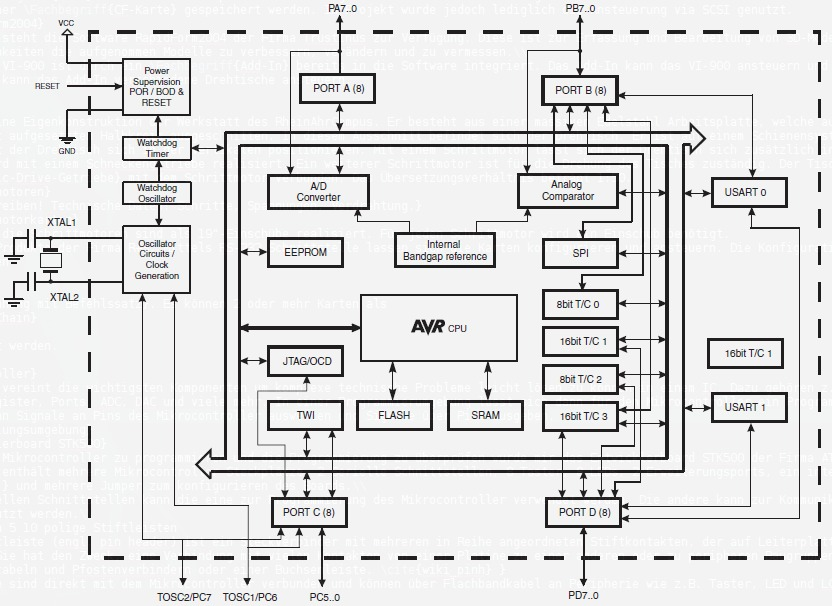
\includegraphics[width=\textwidth]{uC_Block}
\caption{Block Diagram eines Mikrocontroller}
\label{fig:uC Blockdiagramm}
\citep{atmel:ug_324A}
\end{figure}

\subsection{Entwicklerboard STK500}
Um Mikrocontroller zu programmieren und die Programmierung zu überprüfen kann das \Fachbegriff{Entwicklerboard} STK500 der Firma ATMEL verwendet werden. Das Board enthält mehrere Mikrocontroller Steckplätze, 2 Serielle Schnittstellen, 8 Taster, 8 LEDs, 2 Erweiterungsports, ein \Fachbegriff{ISP} \todo{besserer Name!} und mehrere Jumper zum konfigurieren des Boards.\\
Von den beiden seriellen Schnittstellen kann die eine zur Programmierung des Mikrocontroller verwendet werden. Die andere kann zur Kommunikation mit dem Mikrocontroller genutzt werden.\\
Auf dem Board stehen 5 10 polige Stiftleisten 
%\footnote{Eine Stiftleiste (engl. pin header) ist ein Steckverbinder mit mehreren in Reihe angeordneten Stiftkontakten, der auf Leiterplatten in der Elektronik Verwendung findet. Sie hat den Zweck, eine Verbindung mit vielen Kontakten von einer Platine zu einer anderen oder zu peripheren Baugruppen herzustellen, meist mit Hilfe von Flachbandkabeln und Pfostenverbindern oder einer Buchsenleiste. \cite{wiki:Stiftleiste} }
zur Verfügung. Diese sind direkt mit dem Mikrocontroller verbunden und können über Flachbandkabel an Peripherie wie z.B. Taster, LED und LC-Displays angeschlossen werden.

\subsection{AVRISP mkII}
Das AVRISP mkII ist ein USB-basiertes In-System-Programmiersystem. Dieses kann anstelle des RS-232 basierten Programmiersystem des STK500 verwendet werden.\\
Die Übertragungsgeschwindigkeit des AVRISP mkII ist wesentlich höher als die über die Serielle Verbindung. Desweiteren wurde der ATmega324A nicht mehr vom STK500 internen ISP unterstützt.\\
Der AVRISP mkII lässt sich einfach an den Programmierport, eine 6-Polige Stiftleiste, des STK500 anschließen.

\subsection{MAX232}
Die Spannungspegel des Mikrocontroller(typ. 0-5 V) sind nicht kompatibel zu den Spannungspegeln des RS-232 Standards (typ. -12-+12 V). Daher wird der \Fachbegriff{Pegelumsetzer} MAX232 genutzt. Dieser wandelt mit internen Operationsverstärkern die Spannungspegel auf den richtigen Wert.\todo{Beschaltung?}
\section{Platinenlayout}
Für den Mikrocontroller und seine Peripherie wurde ein Platinenlayout entwickelt. Dieses wurde in der Opensource Software KiCad entwickelt. \\ 
Dazu wurden die Schaltungen wie auf dem STK500 in den Schaltplan übernommen und dort das Layout entwickelt. \todo{Schaltplan und Layout Bild einbinden.}